\documentclass{article}
\usepackage{graphicx} % Required for inserting images
\usepackage{float}
\usepackage{hyperref}
\usepackage[inkscapeformat=png]{svg}
\usepackage[margin=0.85in]{geometry}
\usepackage[italian]{babel} % nomi di tabelle e figure ora sono in italiano
\usepackage{changepage}

\hypersetup{
  colorlinks,
  citecolor=black,
  filecolor=black,
  linkcolor=black,
  urlcolor=black
}



\begin{document}

  \begin{titlepage}
    \begin{center}
      \vspace*{1cm}
      
\includegraphics[width=10cm]{unifi.jpg} \\
      \vspace{1cm}
      \LARGE Università degli studi di Firenze \\
      \vspace{0.4cm}
      \LARGE Dipartimento di Ingegneria dell'Informazione \\
      \rule{17cm}{1.5pt} \\
      \vspace{0.4cm}
      \LARGE \textbf{Swetify: un'applicazione a linea di comando per lo streaming musicale} \\
      \rule{17cm}{1.5pt} \\
      \vspace{1cm}
      \begin{adjustwidth}{1cm}{}
        \begin{flushleft}
          \begin{minipage}[t]{0.45\textwidth}
            \large \textit{\textbf{Autori:}} \\
            A. Delli Colli \\
            N. Malgeri \\
            F. Viti \\
            \hspace{-4cm} \\
            \large \textit{\textbf{Anno accademico}:} \\
            2023-2024
          \end{minipage}
          \begin{minipage}[t]{0.45\textwidth}
            \hspace*{1cm}
            \large \textit{\textbf{Corso:}} \\
            \hspace*{1.1cm} B024253 \\
            \hspace*{1.1cm} Basi di dati - Ingegneria del software \\
            \vspace{0.5cm} \\
            \hspace*{1.1cm} \textit{\textbf{Docente del corso:}} \\
            \hspace*{1.1cm} E. Vicario \\
          \end{minipage}
        \end{flushleft}
      \end{adjustwidth}
    \end{center}
  \end{titlepage}

  \renewcommand{\contentsname}{\LARGE Indice}
  \tableofcontents
  \pagebreak


  \section{Introduzione}

  \subsection{Motivazioni}
  Il nostro intensivo utilizzo di piattaforme di streaming musicali ha suscitato in noi un interesse riguardo
  la loro struttura e il desiderio di replicarne il funzionamento.\\
  Abbiamo deciso quindi di realizzare un'applicazione che simuli le loro funzionalità da noi denominata Swetify.

  \subsection{Architettura dell'applicazione e pratiche utilizzate}
  Per la progettazione del software è stato seguito lo standard UML, realizzando i diagrammi con StarUML.
  Il software è stato realizzato in Java. Il modello dei dati è rappresentato dal package \textbf{domainModel},
  mentre la logica e la visualizzazione dell'interfaccia utente si trova nel package \textbf{businessLogic}. La \textbf{businessLogic} si interfaccia con dei DAO che si occupano di rendere i dati persistenti attraverso \textbf{JPA} (\textbf{\textit{Jakarta Persistence API}}). In particolare è stato scelto \textbf{\textit{Hibernate}} come implementazione della \textbf{JPA}. Come RDBMS è stato usato \textbf{H2}, integrato di default in \textbf{\textit{Hibernate}}. L'architettura generale dell'applicazione è illustrata in Figura \ref{fig:architettura}.
  Il testing è stato effettuato con il framework \textbf{\textit{JUnit 5}}.
  Per semplicità, l'interfaccia effettivamente realizzata è a linea di comando.
  Sono stati realizzati dei mockup utilizzando \textbf{\textit{Inkscape}}, un programma per grafica vettoriale, che rappresentano l'aspetto che avrebbe l'applicazione se fosse stata realizzata un'interfaccia grafica.

  \begin{figure}[H]
    \centering
    \includesvg[width=0.7\linewidth]{Architettura.svg}
    \caption{Architettura dell'applicazione}
    \label{fig:architettura}
  \end{figure}


  \section{Requisiti}
  \label{sec:reqFunc}
  Swetify prevede la partecipazione di due tipologie di utenti: cliente e artista.

  \subsection{Funzionalità proposte per il cliente}

  \begin{itemize}

    \item visualizzare un catalogo musicale che consenta agli utenti di cercare brani, album e artisti tramite una barra
    di ricerca.

    \item visualizzare le informazioni dettagliate di un brano, inclusi titolo, artista, album e durata.

    \item riprodurre, mettere in pausa e saltare i brani.

    \item creare, modificare ed eliminare le proprie playlist, aggiungere e rimuovere brani da queste playlist.

    \item ricevere raccomandazioni di brani basate sulla cronologia di ascolto dell'utente

    \item seguire gli artisti per ricevere aggiornamenti sui nuovi rilasci.

  \end{itemize}

  \subsection{Funzionalità proposte per l'artista}

  \begin{itemize}

    \item caricare album contenenti canzoni o podcast.

  \end{itemize}


  \section{Progettazione}

  \subsection{Diagramma dei casi d'uso}

  Come accennato nella sezione \ref{sec:reqFunc}, ci sono due protagonisti, l'utente (\textbf{\textit{Customer}}) e l'artista (\textbf{\textit{Artist}}). La figura \ref{fig:useCaseDiagram} rappresenta il diagramma dei casi d'uso, questi ultimi corrispondenti ai requisiti funzionali descritti precedentemente.

  \begin{figure}[H]
    \centering
    \includesvg[width=0.7\linewidth]{UseCaseDiagram.svg}
    \caption{diagramma dei casi d'uso}
    \label{fig:useCaseDiagram}
  \end{figure}

  \subsection{Template dei casi d'uso}

  \begin{table}[H]
    \centering
    \begin{tabular}{|l|l|}
      \hline
      \textbf{UC1}            & \textbf{riproduzione canzone}                                                 \\
      \hline
      livello                 & user goal                                                                     \\
      \hline
      descrizione             & l'utente cerca e riproduce una canzone                                        \\
      \hline
      attori                  & cliente                                                                       \\
      \hline
      pre-condizioni          & l'utente deve avere le credenziali per effettuare l'accesso                   \\
      \hline
      post-condizioni         & la canzone selezionata viene aggiunta alla coda                               \\
      \hline
      normale svolgimento     & 1) l'utente apre la pagina di ricerca (mockup in figura \ref{fig:searchPage}) \\
      & 2) inserisce il nome di una canzone                                           \\
      & 3) seleziona una voce dall'elenco proposto                                    \\
      & 4) seleziona l'opzione ``aggiungi in coda"

      \\
      \hline
      svolgimenti alternativi & 4b) l'utente seleziona l'opzione "aggiungi in testa"                          \\
      \hline
    \end{tabular}
    \label{tab:uct1}
  \end{table}

  \vspace{40pt}

  \begin{table}[H]
    \centering
    \begin{tabular}{|l|l|}
      \hline
      \textbf{UC2}            & \textbf{modifica playlist}                                  \\
      \hline
      livello                 & user goal                                                   \\
      \hline
      descrizione             & l'utente modifica una delle sue playlist personali          \\
      \hline
      attori                  & cliente                                                     \\
      \hline
      pre-condizioni          & l'utente deve avere le credenziali per effettuare l'accesso \\
      & ed avere una playlist salvata                               \\
      \hline
      post-condizioni         & la playlist presenta i cambiamenti apportati dall'utente    \\
      \hline
      normale svolgimento     & 1) l'utente apre la pagina "le mie playlist"                \\
      & 2) l'utente seleziona la playlist da modificare             \\
      & 3) l'utente cerca una canzone da aggiungere                 \\
      & 4) l'utente termina salvando le modifiche

      \\
      \hline
      svolgimenti alternativi & 3b) l'utente seleziona una canzone da rimuovere             \\
      & 4b) l'utente annulla le modifiche alla playlist             \\
      \hline

    \end{tabular}
    \label{tab:uct2}
  \end{table}

  \vspace{40pt}

  \begin{table}[H]
    \centering
    \begin{tabular}{|l|l|}
      \hline
      \textbf{UC3}            & \textbf{aggiunta album}                                      \\
      \hline
      livello                 & user goal                                                    \\
      \hline
      descrizione             & l'artista carica un nuovo album sul suo profilo              \\
      \hline
      attori                  & artista                                                      \\
      \hline
      pre-condizioni          & l'artista deve avere le credenziali per effettuare l'accesso \\
      \hline
      post-condizioni         & il nuovo album è visibile se cercato dagli utenti            \\
      \hline
      normale svolgimento     & 1) l'artista seleziona l'opzione carica album                \\
      & 2) inserisce i nomi delle canzoni ed i rispettivi dati       \\
      & 3) l'artista termina l'inserimento salvando l'album
      \\
      \hline
      svolgimenti alternativi & 3b) l'artista annulla il caricamento dell'album              \\
      \hline

    \end{tabular}
    \label{tab:uct3}
  \end{table}

  \vspace{40pt}

  \begin{table}[H]
    \centering
    \begin{tabular}{|l|l|}
      \hline
      \textbf{UC4}                     & \textbf{iscrizione ad un artista}                           \\
      \hline
      livello                          & function                                                    \\
      \hline
      descrizione                      & l'utente aggiunge un artista agli artisti seguiti           \\
      \hline
      attori                           & cliente                                                     \\
      \hline
      pre-condizioni                   & l'utente deve avere le credenziali per effettuare l'accesso \\
      \hline
      post-condizioni                  & nel momento in cui l'artista carica un nuovo album          \\
      & l'utente può visualizzarlo nella sezione                    \\
      & "nuovi rilasci"                                             \\
      \hline
      normale svolgimento \hspace{5pt} & 1) l'utente apre la pagina di ricerca                       \\
      & 2) inserisce il nome di una canzone                         \\
      & 3) seleziona una voce dall'elenco proposto                  \\
      & 4) seleziona l'opzione ``aggiungi in coda"
      \\
      \hline
    \end{tabular}
    \label{tab:uct4}
  \end{table}

  \vspace{40pt}

  \begin{table}[H]
    \centering
    \begin{tabular}{|l|l|}
      \hline
      \textbf{UC5}                     & \textbf{visualizzazione dei consigliati}                                         \\
      \hline
      livello                          & user goal                                                                        \\
      \hline
      descrizione                      & l'utente visualizza le canzoni ed i podcast consigliati                          \\
      \hline
      attori                           & cliente                                                                          \\
      \hline
      pre-condizioni                   & l'utente deve avere le credenziali per effettuare l'accesso                      \\
      & e avere ascoltato almeno una canzone o podcast                                   \\
      \hline
      post-condizioni                  & i consigliati sono mostrati nella sezione apposita                               \\
      \hline
      normale svolgimento \hspace{5pt} & 1) l'utente va alla homepage                                                     \\
      & 2) accede alla sezione dei consigliati                                           \\
      & 3) visualizza le tracce consigliate (mockup in figura \ref{fig:suggestionsPage}) \\
      \hline
    \end{tabular}
    \label{tab:uct5}
  \end{table}

  \pagebreak

  \subsection{Mockups}

  \subsubsection{Pagina di accesso}
  \begin{figure}[H]
    \centering
    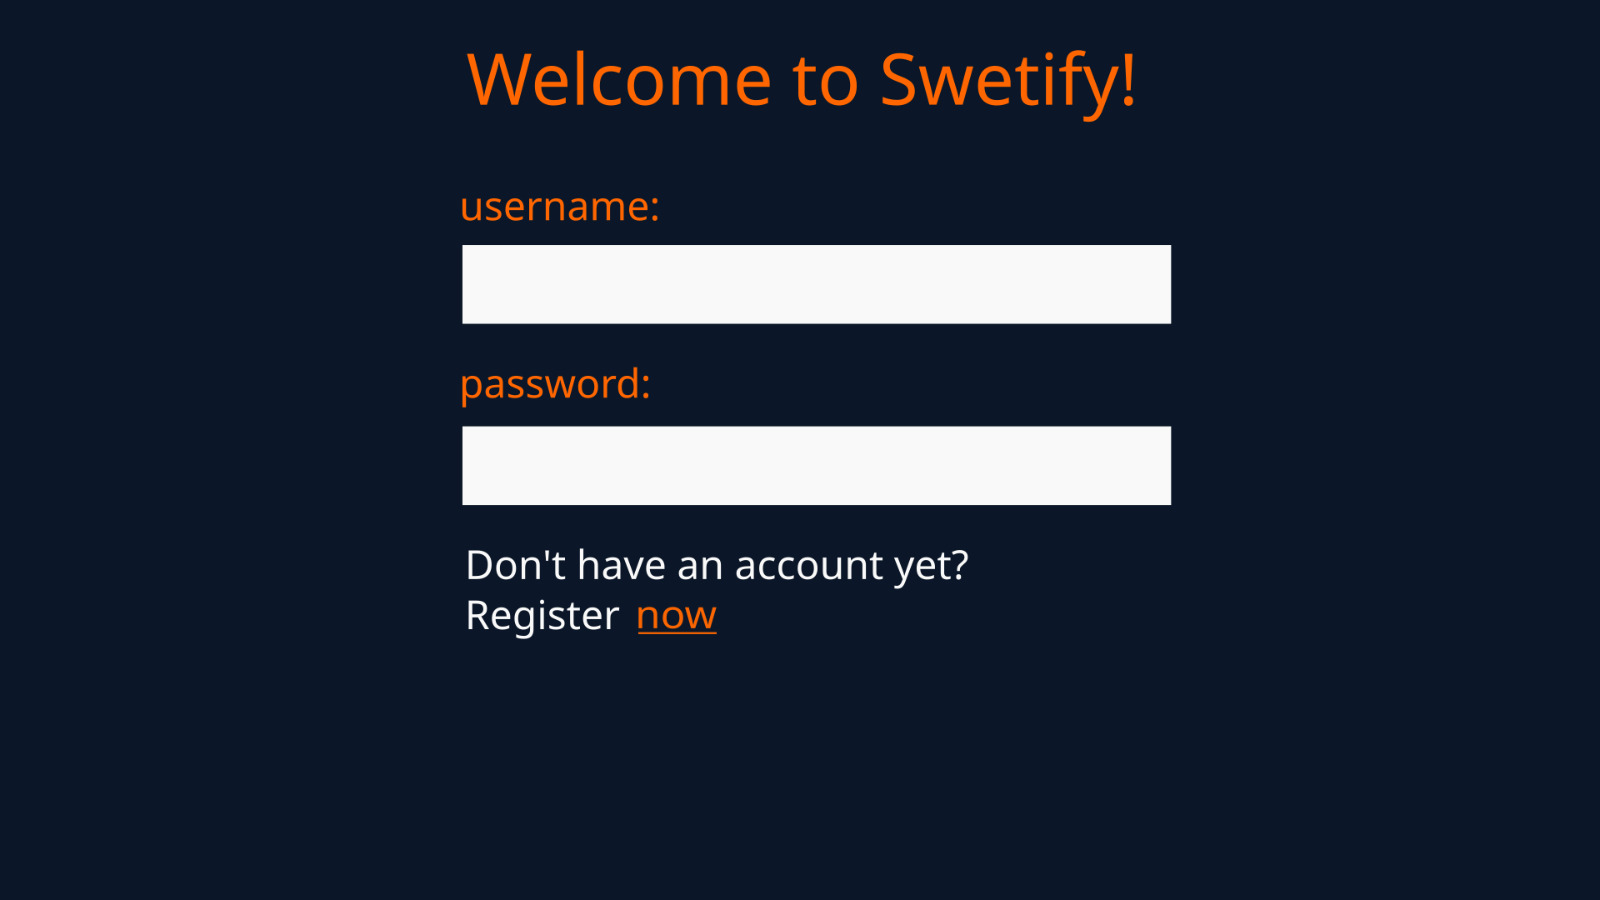
\includegraphics[scale=0.25]{welcome}
    \caption{prototipo della pagina di login}
    \label{fig:loginPage}
  \end{figure}

  \subsubsection{Pagina di ricerca}
  \begin{figure}[H]
    \centering
    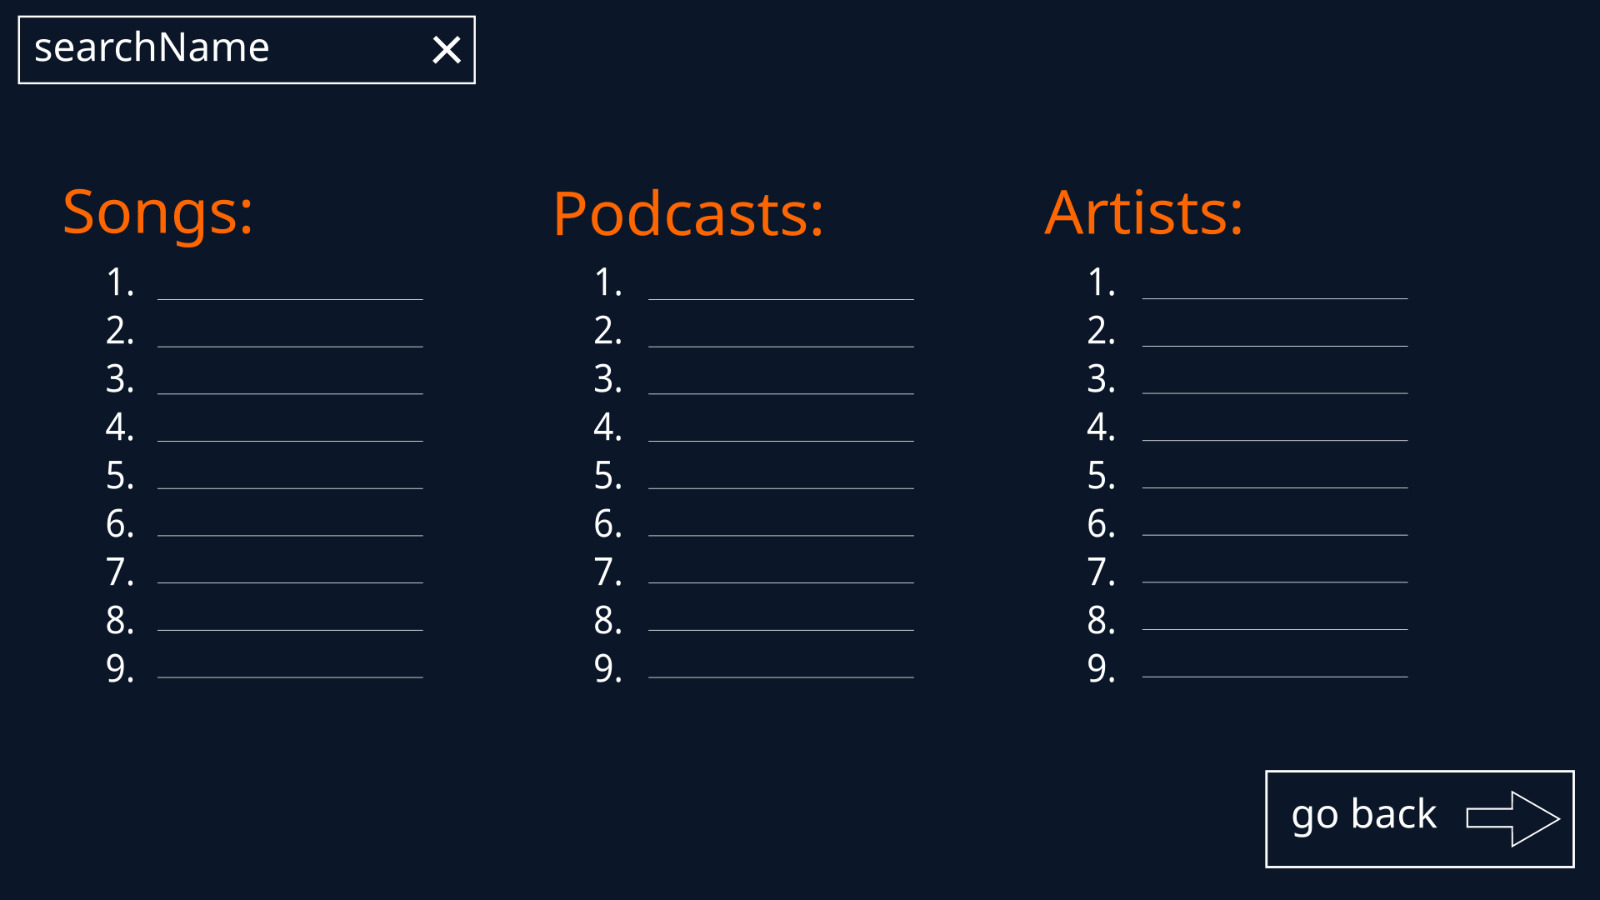
\includegraphics[scale=0.25]{search}
    \caption{prototipo della pagina di ricerca}
    \label{fig:searchPage}
  \end{figure}

  \subsubsection{Suggerimenti}
  \begin{figure}[H]
    \centering
    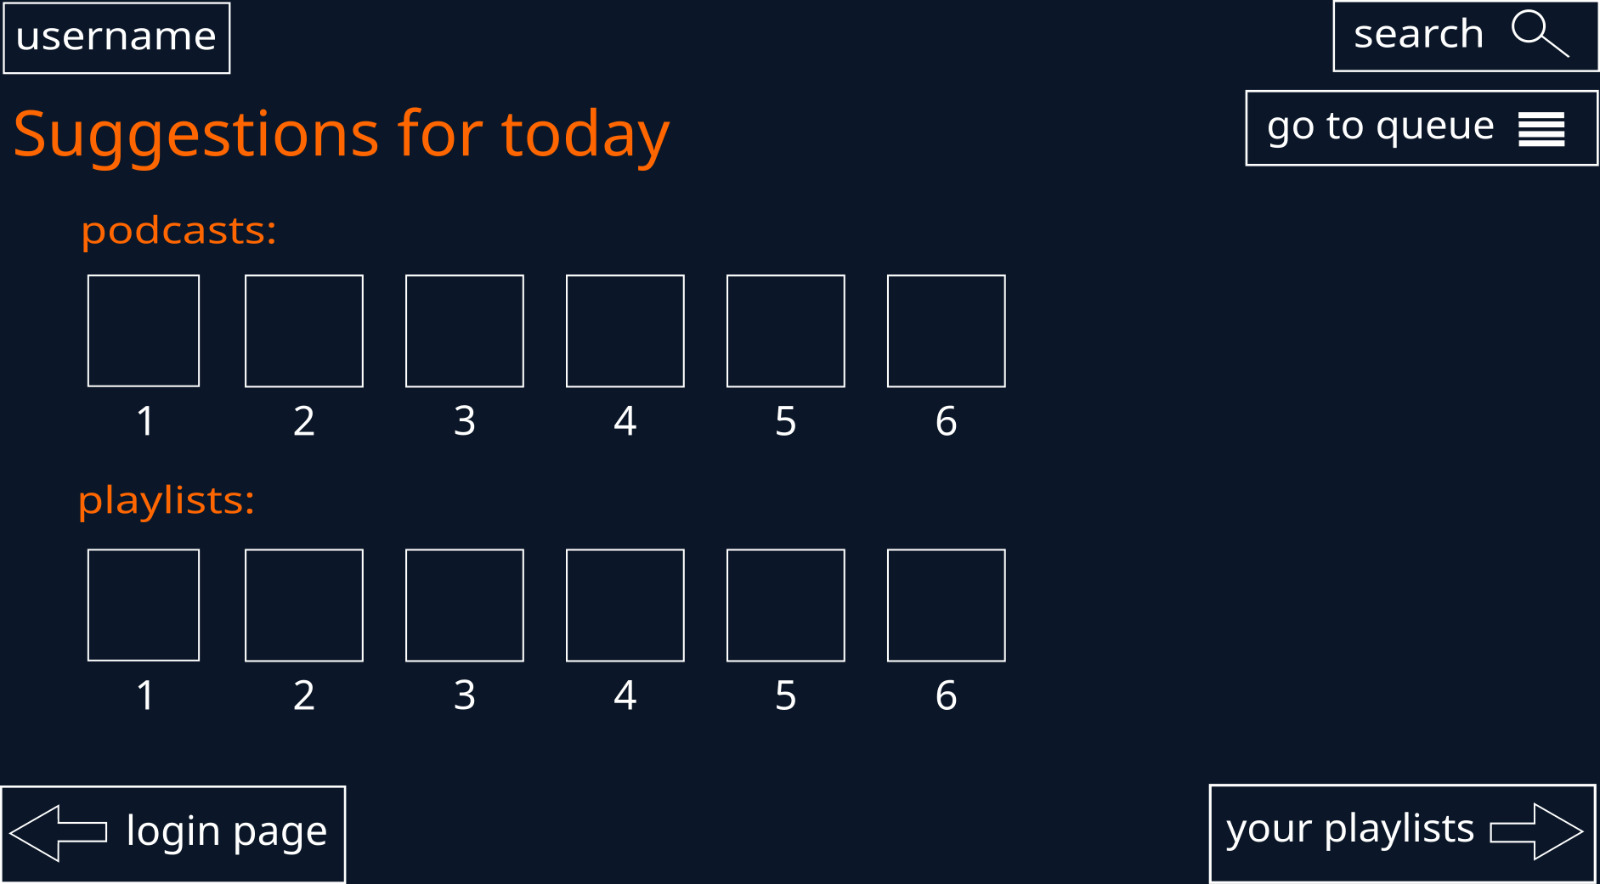
\includegraphics[scale=0.25]{suggestions}
    \caption{prototipo della pagina dei consigliati}
    \label{fig:suggestionsPage}
  \end{figure}

  \subsubsection{Coda di riproduzione}
  \begin{figure}[H]
    \centering
    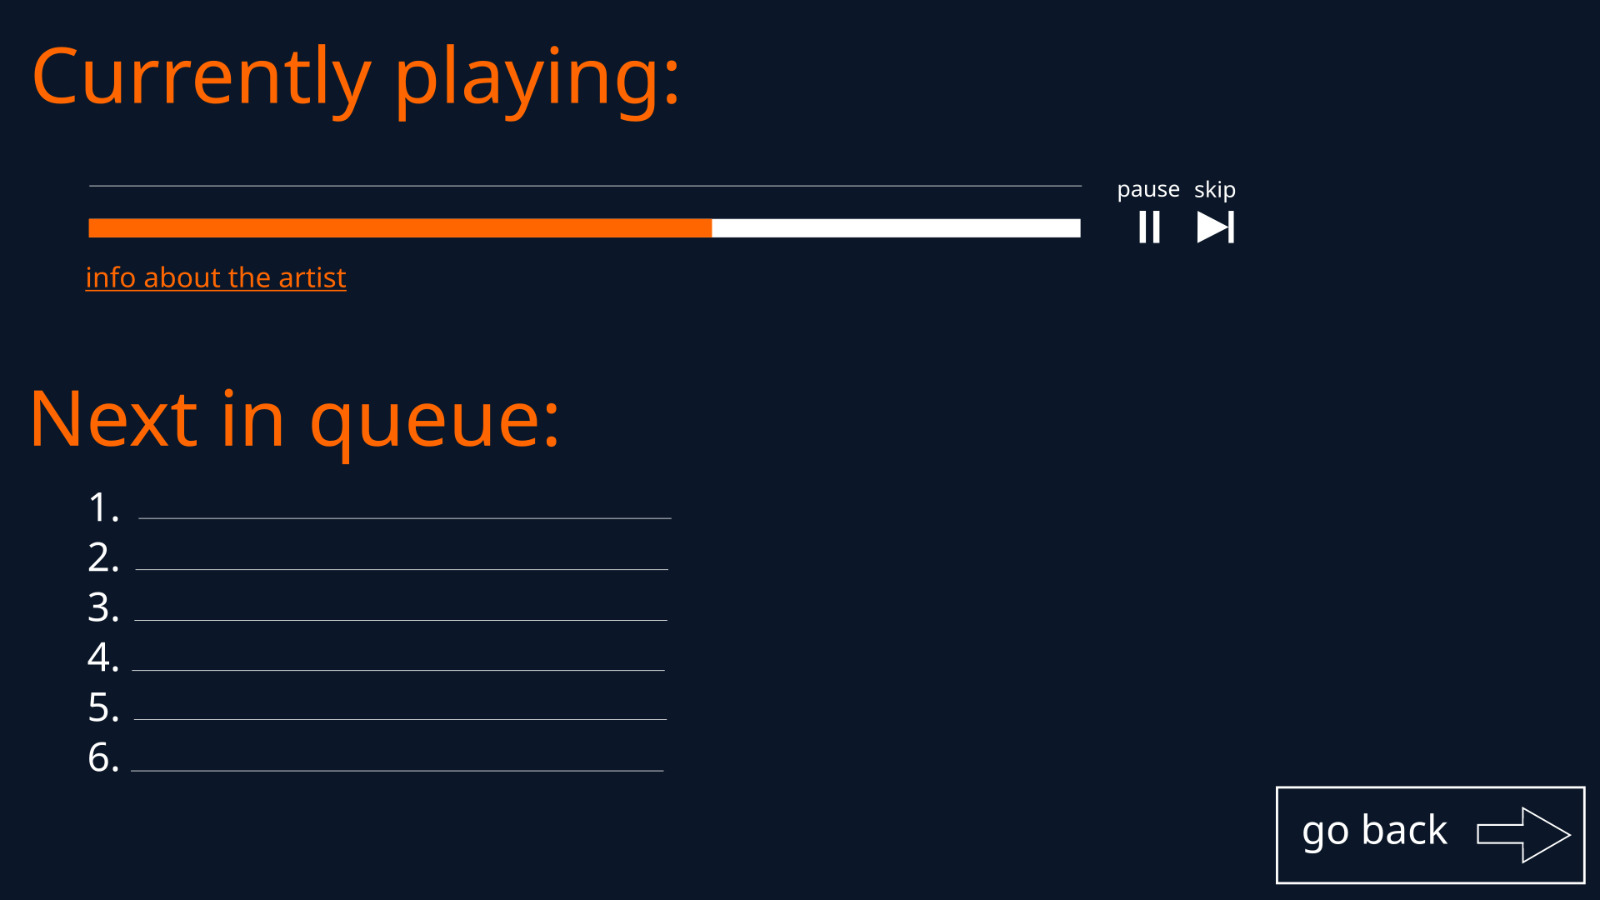
\includegraphics[scale=0.25]{playback}
    \caption{prototipo della coda di riproduzione}
    \label{fig:playbackQueue}
  \end{figure}

  \subsection{Struttura delle classi}

  \subsubsection{Domain model}
  \begin{figure}[H]
    \centering
    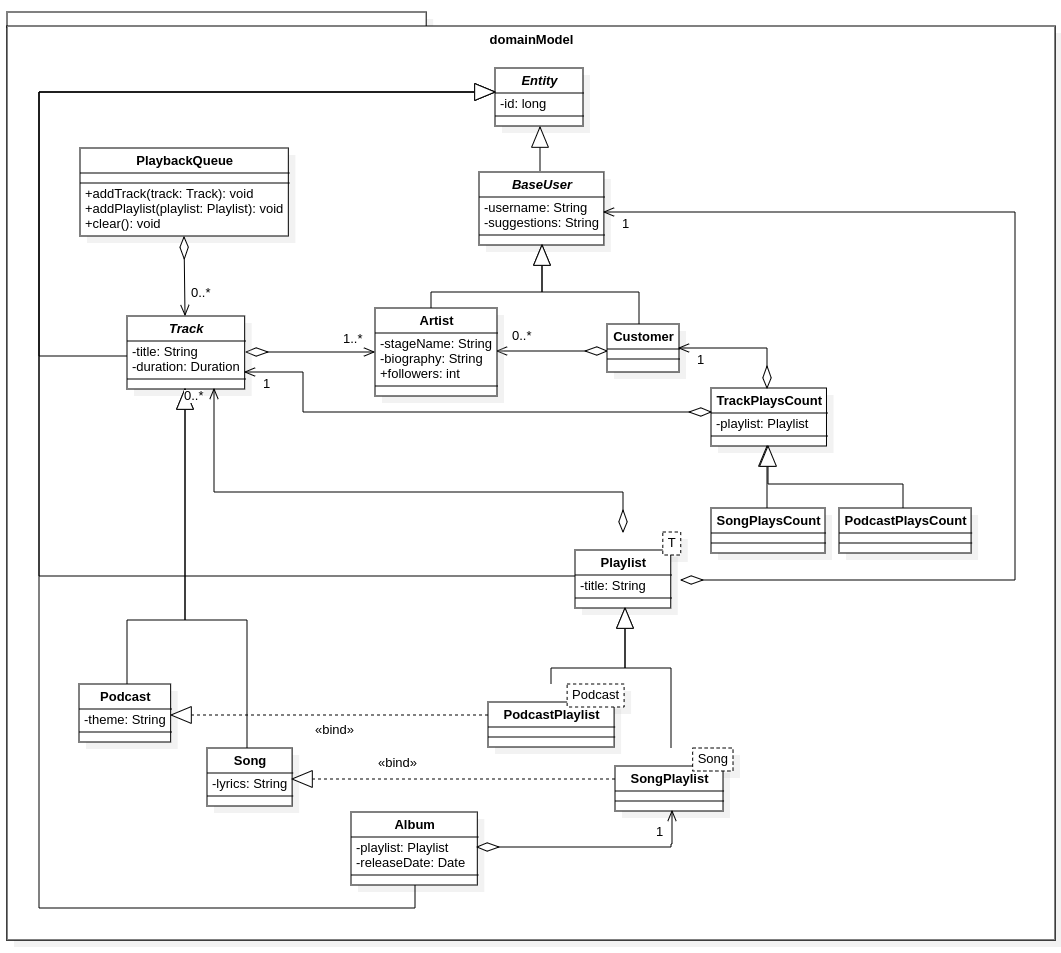
\includegraphics[width=0.9\linewidth]{domainModel.png}
    \caption{diagramma delle classi contenute nel package \textit{domainModel}}
    \label{fig:domainModel}
  \end{figure}

  Definisce la rappresentazione dei dati all'interno dell'applicazione e come gli oggetti sono mappati nel database. Per fare questo è stata usata la tecnica ORM (Object Relational Mapping), realizzata tramite l'utilizzo delle annotazioni fornite dalle JPA (package jakarta.persistence).

  \subsubsection{Business logic}

  \begin{figure}[H]
    \centering
    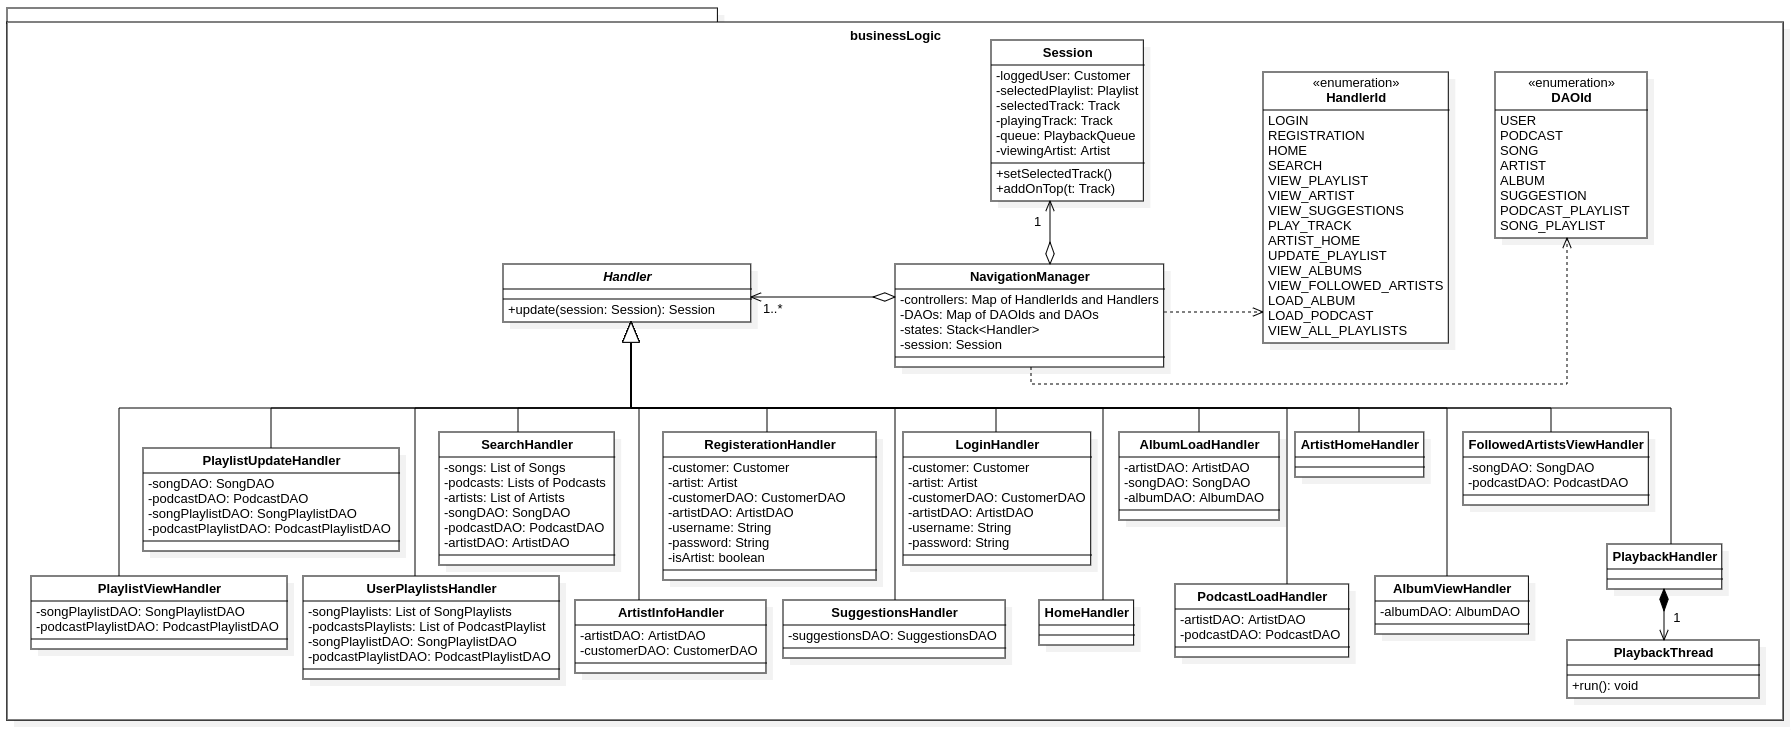
\includegraphics[width=1\linewidth]{businessLogic.png}
    \caption{diagramma delle classi contenute nel package \textit{businessLogic}}
    \label{fig:businessLogic}
  \end{figure}

  Definisce le regole, i processi e le funzionalità che guidano il comportamento dell’applicazione, in base alle diverse esigenze degli utenti. All'interno del package \textbf{\textit{businessLogic}} (figura \ref{fig:businessLogic}) sono presenti le classi che si occupano della visualizzazione, da linea di comando, del contenuto delle finestre dell'applicazione; queste classi sono dette \textit{Handlers} (come ad esempio \textit{HomeHandler} per la visualizzazione della homepage, \textit{SearchHandler} per la finestra di ricerca). Il passaggio da una finestra all'altra viene gestito dalla classe \textbf{\textit{NavigationManager}}.

  \subsubsection{DAO}
  \begin{figure}[H]
    \centering
    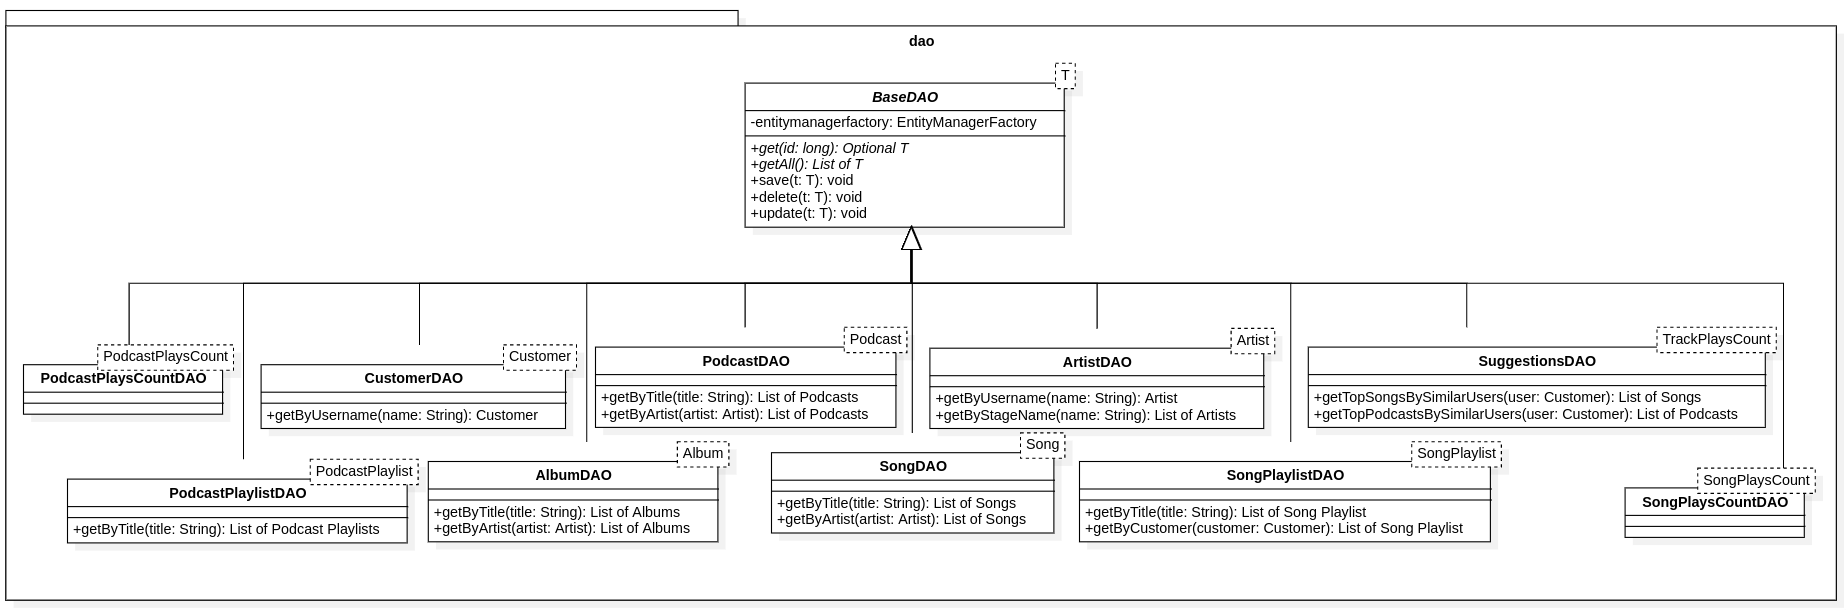
\includegraphics[width=1\linewidth]{DAOs.png}
    \caption{diagramma delle classi contenute nel package \textit{dao}}
    \label{fig:DAO}
  \end{figure}
  Contiene le classi che realizzano il Data Access Object pattern che si occupa della persistenza dei dati.

  \subsection{Design patterns}

  \subsubsection{DAO}
  \begin{figure}[H]
    \centering
    \includesvg[width=0.85\linewidth]{DAOPattern.svg}
    \caption{diagramma delle classi del design pattern DAO}
    \label{fig:daoPattern}
  \end{figure}
  Il DAO (Data Access Object) è un pattern strutturale che permette di disaccoppiare il layer di business logic da quello che si occupa di rendere gli oggetti persistenti nel database. I DAO espongono alla business logic un'API per effettuare le operazioni di CRUD. Ciò permette di rispettare il principio di singola responsabilità.
  Nel nostro caso, è stato prevista una classe base astratta e generica che definisce l'implementazione di default per le operazioni CRUD di base. Nella maggior parte dei casi questa implementazione è adeguata per tutti i DAO concreti. Nei casi in cui erano necessari metodi di accesso ai dati più specifici, ad esempio filtraggio per attributi che non siano l'ID, essi sono stati implementati nel rispettivo DAO concreto.

  \subsubsection{State}
  \label{sec:statePattern}

  \begin{figure}[H]
    \centering
    \includesvg[width=0.8\linewidth]{StatePattern.svg}
    \caption{State pattern}
    \label{fig:statePattern}
  \end{figure}

  Lo \textit{State} è un pattern comportamentale, mostrato in figura \ref{fig:statePattern}, che permette ad un oggetto di cambiare comportamento sulla base di un proprio stato. Ha tre componenti principali:
  \begin{itemize}
    \item \textbf{\textit{State}}: classe base astratta rappresentante uno stato generico dell'oggetto. Espone un metodo \textbf{\textit{handle()}} implementato dalle classi derivate
    \item \textbf{\textit{ConcreteState}}: classe concreta derivata da \textit{State} rappresentante uno specifico stato che l'oggetto può assumere
    \item \textbf{\textit{Context}}: rappresenta l'oggetto il cui comportamento dipende dallo stato che possiede; ha un riferimento a \textbf{\textit{State}} e un metodo \textbf{\textit{request()}}, per l'aggiornamento dello stato
  \end{itemize}

  Quando un oggetto di tipo \textit{Context} deve mostrare un determinato comportamento, viene chiamato il metodo \textit{request()} che internamente chiama \textit{State.handle()} e delega tale responsabilità allo stato corrente dell'oggetto, di tipo \textit{ConcreteState}. Se in un qualsiasi momento avviene una transizione ad un altro \textit{ConcreteState}, il \textit{Context} aggiornerà il proprio riferimento e ciò si riflette in un cambiamento dello stato interno.

  Lo state pattern si può ritrovare nelle classi rappresentanti gli \textit{Handler} all'interno del package \textit{businessLogic} (figura \ref{fig:businessLogic}). Infatti, la classe \textit{NavigationManager} può essere vista come un \textit{Context} il cui comportamento dipende dall'\textit{Handler} "attivo" nell'applicazione (\textit{ConcreteState}); dettagli maggiori sull'implementazione sono presenti nella sezione \ref{sec:navManager}

  \subsection{Diagramma di sequenza}

  \begin{figure}[H]
    \centering
    \includesvg[width=0.85\linewidth]{ModifyUserPlaylist.svg}
    \caption{diagramma di sequenza relativo alla modifica della playlist di un utente}
    \label{fig:seqDiag}
  \end{figure}

  Un \textbf{diagramma di sequenza} mostra la successione temporale delle chiamate dei metodi delle classi dell'applicazione in un determinato scenario di utilizzo. La figura \ref{fig:seqDiag} rappresenta il diagramma di sequenza relativo allo scenario in cui un utente decide di modificare una delle proprie playlist.


  \section{Implementazione}

  \subsection{Domain model}

  \subsubsection{BaseEntity}
  Classe base astratta che garantisce la presenza di un ID in tutte entità concrete.
  \subsubsection{BaseUser}
  Classe base per Customer e Artist che contiene le credenziali di accesso.
  \subsubsection{Customer}
  Estende il BaseUser aggiungendo una lista di artisti seguiti.
  \subsubsection{Artist}
  Estende il BasUser aggiungendo il nome d'arte, la biografia e il numero di follower.
  \subsubsection{Track}
  Rappresenta una traccia audio che può essere aggiunta alla coda\\ di riproduzione.

  \subsubsection{DurationConverter}
  Implementa l'interfaccia AttributeConverter di Jakarta per convertire la durata delle Track dal tipo Duration a un tipo supportato dal DBMS.
  \subsubsection{Song}
  Concretizzazione di Track che rappresenta una canzone.
  \subsubsection{Podcast}
  Concretizzazione di Track che rappresenta un podcast.
  \subsubsection{Playlist}
  Rappresenta una playlist generica ed espone i metodi per aggiungere o rimuovere\\ delle track in testa oppure in coda.

  \subsubsection{SongPlaylist}
  Rappresenta una playlist a cui possono essere aggiunte soltanto canzoni.

  \subsubsection{PodcastPlaylist}
  Rappresenta una playlist a cui possono essere aggiunti soltanto podcast.
  \subsubsection{Album}
  Incapsula una playlist di cui espone selettivamente soltanto i metodi di lettura, in modo da rendere immutabile la lista di canzoni dopo che è stata creata.
  \subsubsection{PlaybackQueue}
  Rappresenta la coda di riproduzione e permette di aggiungere in testa ed in coda oltre ad eliminare in testa. Non è persistente.

  \subsubsection{TrackPlaysCount}
  Classe astratta che associa un Customer a ogni Track che ha ascoltato mantenendo un conteggio del numero di riproduzioni. Questa informazione serve per il calcolo delle tracce suggerite.

  \subsubsection{SongPlaysCount}
  Concretizzazione di TrackPlaysCount che conta quante volte un utente ha riprodotto ogni canzone

  \subsubsection{PodcastPlaysCount}
  Concretizzazione di TrackPlaysCount che conta quante volte un utente ha riprodotto ogni canzone

  \subsubsection{TrackPlaysCountListener}
  Trigger che mantiene aggiornato il numero totale di riproduzioni di una traccia.

  \subsection{Business logic}

  \subsubsection{Handler}
  Classe base astratta che rappresenta un \textit{Handler} generico e corrisponde alla classe \textit{State} dello State pattern (sezione \ref{sec:statePattern}). Ha un metodo \textit{update()} per aggiornare ciò che viene visualizzato da linea di comando come finestra corrente dell'applicazione, definito all'interno delle classi derivate.

  \subsubsection{Session}
  Classe che rappresenta una sessione dell'applicazione; permette ai vari \textit{Handler} di comunicare tra loro dati come l'utente che ha effettuato l'accesso, la canzone o la playlist selezionata

  \subsubsection{NavigationManager}
  \label{sec:navManager}
  Gestisce la navigazione tra le pagine passando il controllo ai vari handler; rappresenta il \textit{Context} dello State pattern (sezione \ref{sec:statePattern}). Ha uno stack di riferimenti a \textit{Handler} chiamato \textit{states}, attraverso il quale viene tenuta traccia della finestra visualizzata in un certo momento. Il metodo \textit{switchToController()} (figura \ref{fig:switchToController}) effettua un \textit{push} sullo stack dell'\textit{Handler} a cui deve essere passato il controllo. \textit{NavigationManager.switchToController()} si trova all'interno dell' \textit{update()} di ciascun \textit{Handler}, metodo che viene eseguito all'interno di un loop nella \textit{run()} del \textit{NavigationManager} (figura \ref{fig:run})

  \begin{figure}[H]
    \centering
    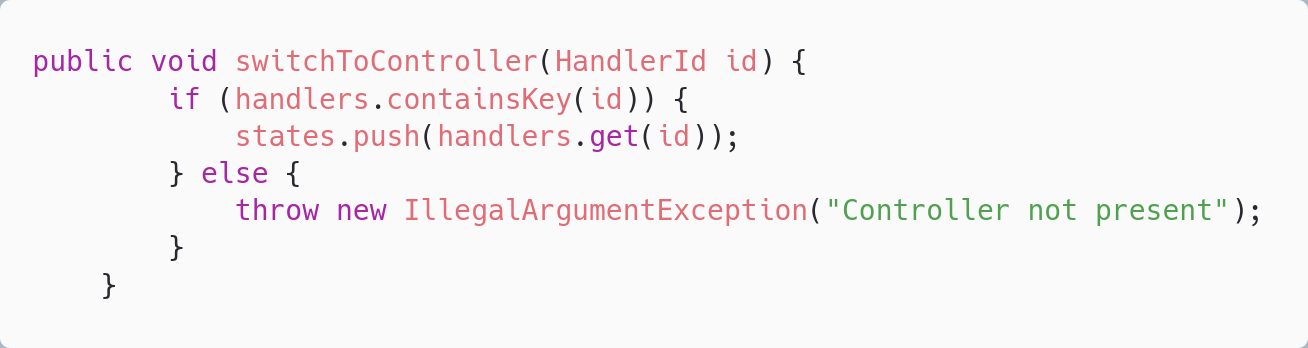
\includegraphics[width=0.8\linewidth]{switchToController.png}
    \caption{metodo \textit{switchToController()} di \textit{NavigationManager}}
    \label{fig:switchToController}
  \end{figure}

  \begin{figure}[H]
    \centering
    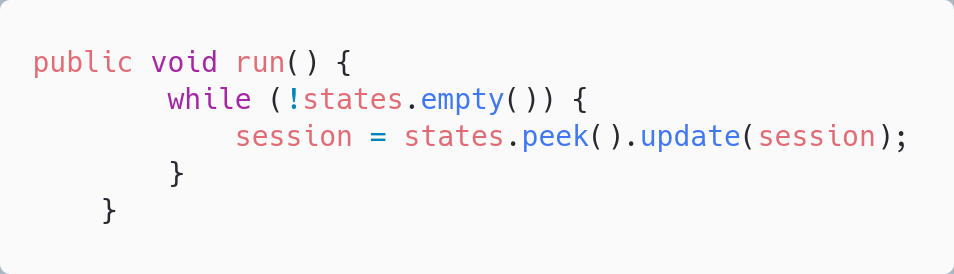
\includegraphics[width=0.8\linewidth]{run.png}
    \caption{metodo \textit{run()} di \textit{NavigationManager}}
    \label{fig:run}
  \end{figure}

  \subsubsection{AlbumViewHandler}
  Permette di visualizzare o riprodurre un album.
  \subsubsection{ArtistInfoHandler}
  Mostra le informazioni salienti di un artista.
  \subsubsection{HomeHandler}
  Contiene la schermata di ingresso e instrada l'utente verso le varie pagine.
  \subsubsection{LoginHandler}
  Permette all'utente di effettuare l'accesso con un nome utente e una password o
  eventualmente passare alla schermata di registrazione.

  \subsubsection{PlaybackHandler}
  Gestisce la coda di riproduzione e permette all'utente di visualizzare i brani contenuti in essa. Utilizza un \textit{thread} che viene fatto partire all'apertura della coda di riproduzione, e che si occupa della visualizzazione della \textit{progress bar} della canzone in cima alla coda.
  In figura \ref{fig:thread} viene mostrato il metodo \textit{run()} del thread della coda di riproduzione.

  \begin{figure}[H]
    \centering
    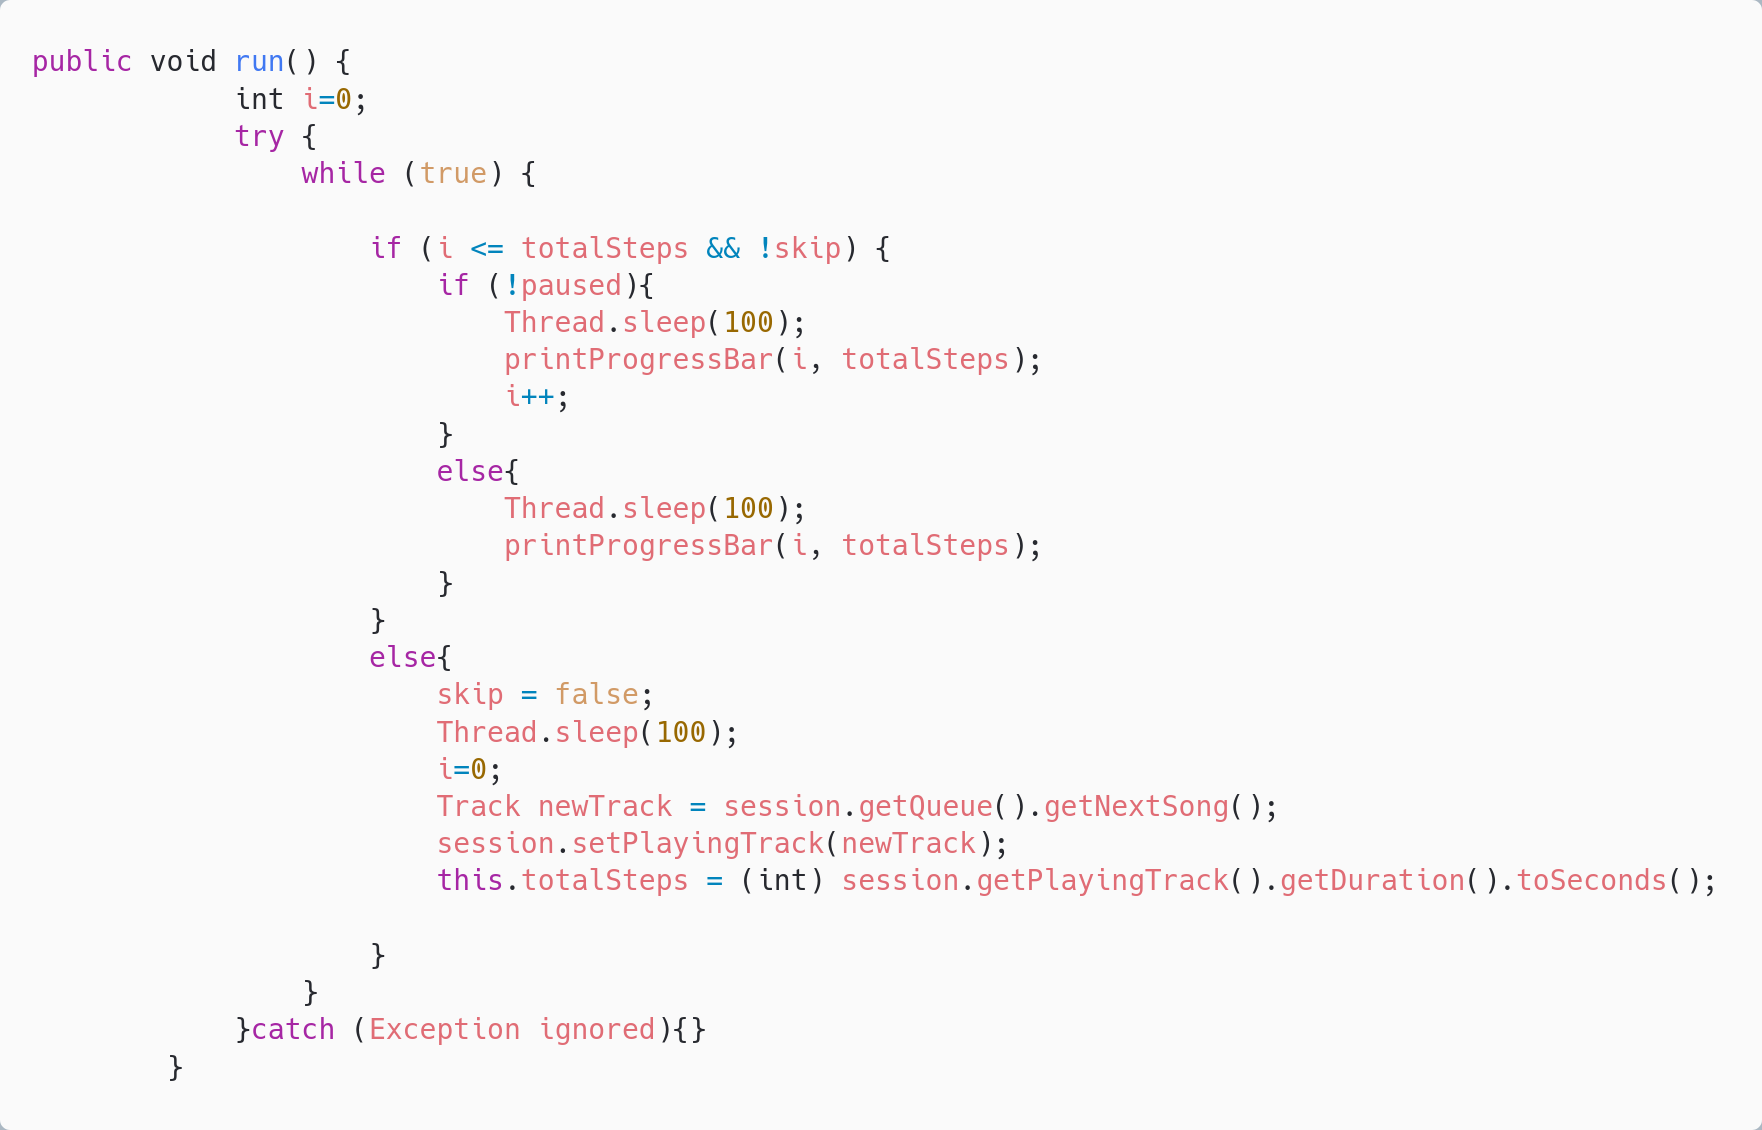
\includegraphics[width=0.8\linewidth]{threadRun.png}
    \caption{metodo \textit{run()} del thread della coda di riproduzione}
    \label{fig:thread}
  \end{figure}



  \subsubsection{PlaylistHandler}
  Mostra all'utente i brani contenuti in una data playlist e permette ad esso di
  aggiungerla alla coda di riproduzione.
  \subsubsection{RegistrationHandler}
  Permette all'utente di registrarsi all'interno dell'applicazione con un
  nome utente ed una password.
  \subsubsection{SearchHandler}
  Gestisce la ricerca all'interno delle canzoni, dei podcast e degli artisti disponibili.
  \subsubsection{SuggestionsHandler}
  Mostra all'utente le tracce consigliate dall'applicazione sulla base dei suoi ultimi ascolti.
  \subsubsection{UserPlaylistsHandler}
  Mostra l'elenco delle playlist create dall'utente.

  \subsection{DAO}

  \subsubsection{BaseDAO}
  Classe base generica del Data Access Object che definisce le operazioni CRUD di base per interfacciarsi col DBMS e ne fornisce un'implementazione di default.
  Metodi implementati:
  \begin{itemize}
    \item \textbf{\textit{get(long id)}}: restituisce un oggetto di tipo T il cui ID nel database corrisponde a quello dato.
    \item \textbf{\textit{getAll()}}: restituisce tutti gli oggetti di tipo T nel database.
    \item \textbf{\textit{save(T t)}}: rende persistente l'oggetto dato.
    \item \textbf{\textit{update(T t)}}: aggiorna nel database lo stato dell'oggetto.
    \item \textbf{\textit{delete(T t)}}: elimina dal database l'oggetto.
  \end{itemize}
  I metodi per eseguire filtraggi sulla base di parametri specifici sono definiti nelle classi derivate.

  \subsubsection{CustomerDAO}
  Permette di ottenere oggetti Customer dal database a patire dal loro username.

  \subsubsection{ArtistDAO}
  Permette di ottenere oggetti Artist dal database a patire dal loro nome d'arte o username.

  \subsubsection{SongDAO}
  Permette di ottenere oggetti Song dal database a partire da una parola chiave o un Artist.

  \subsubsection{PodcastDAO}
  Permette di ottenere oggetti Podcast dal database a partire da una parola chiave o un Artist.

  \subsubsection{SongPlaylistDAO}
  Permette di ottenere oggetti SongPlaylist dal database a partire dal titolo.

  \subsubsection{PodcastPlaylistDAO}
  Permette di ottenere oggetti PodcastPlaylist dal database a partire dal titolo.

  \subsubsection{AlbumDAO}
  Permette di ottenere oggetti Album dal database a partire dal titolo o dall'autore

  \subsubsection{SongPlaysCountDAO}
  Permette di aggiornare nel database il conteggio delle riproduzioni di una canzone.

  \subsubsection{PodcastPlaysCountDAO}
  Permette di aggiornare nel database il conteggio delle riproduzioni di un podcast.

  \subsubsection{SuggestionDAO}
  Permette, dato un utente, di ottenere una lista di canzoni suggerite in base a cosa hanno ascoltato utenti con preferenze affini. Il sistema di suggerimenti propone ad ogni utente delle canzoni che potrebbe apprezzare cercando le canzoni più ascoltate da utenti "simili" a lui.
  Gli utenti sono considerati simili all'utente corrente se hanno ascoltato le sue canzoni più ascoltate.
  Il funzionamento dettagliato del processo è descritto dalla seguente query:
  \begin{figure}
    \centering
    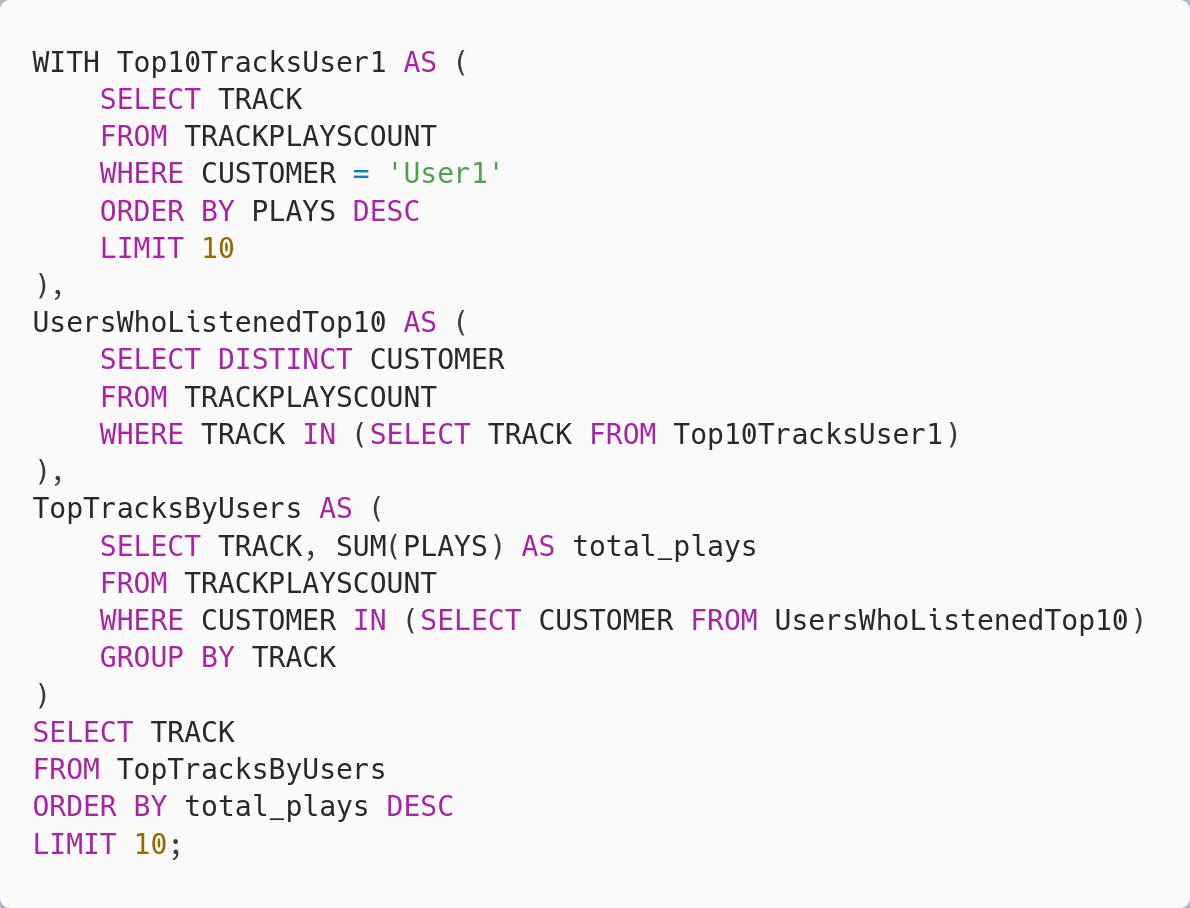
\includegraphics[width=0.7\linewidth]{query.png}
    \caption{Query SQL che restituisce le canzoni suggerite all'utente}
    \label{fig:query}
  \end{figure}


  \section{Test}

  \subsection{Tipologie di test effettuati e organizzazione}

  Per poter garantire il corretto funzionamento di \textit{Swetify} sono stati effettuate due tipologie di test:
  \begin{itemize}
    \item \textbf{test di integrazione}: verificano il comportamento che le componenti dell'applicazione mostrano quando interagiscono tra di loro; nello specifico, vengono testate le operazioni che i DAO utilizzano per interagire con il database di sistema
    \item \textbf{test funzionali}: verificano il comportamento delle singole componenti dell'applicazione in un possibile scenario reale in cui quest'ultima viene utilizzata. Tra i test funzionali rientrano, per esempio, quelli relativi alla navigazione tra una schermata e l'altra dell'applicazione
  \end{itemize}

  \begin{figure}[H]
    \centering
    \includesvg[width=0.85\linewidth]{TestsUML.svg}
    \caption{struttura del package \textit{Test}}
    \label{fig:testsUML}
  \end{figure}

  In figura \ref{fig:testsUML} viene mostrata l'organizzazione delle classi di test, contenute nel package \textit{Test}. Come si può notare, è presente una classe base \textbf{\textit{BaseTest}} contenente le funzionalità comuni a tutte le altre classi, come la funzione \textbf{\textit{setUp()}}; questa funzione serve per ripulire il database tra un test e l'altro, motivo per il quale viene eseguita prima di ciascun test.

  \begin{figure}[H]
    \centering
    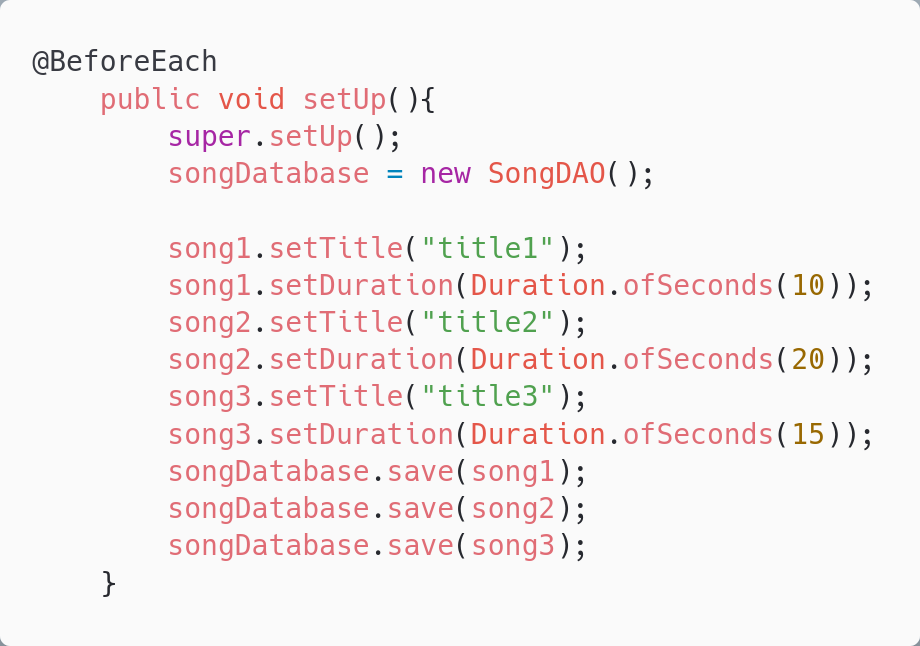
\includegraphics[width=0.5\linewidth]{setUp.png}
    \caption{esempio di implementazione di \textit{setUp()} (in questo caso relativa a SongDAOTest)}
    \label{fig:setUp}
  \end{figure}


  Come si può vedere in figura \ref{fig:setUp}, la \textit{setUp()} della classe base viene chiamata all'inizio della \textit{setUp()} delle classi
  derivate, seguita dall'inizializzazione del database e degli oggetti necessari per l'esecuzione dei test.

  \subsection{Test di integrazione}
  Di seguito vengono descritti i metodi presenti nelle classi relative ai test di integrazione; ogni metodo consiste nel verificare il comportamento di una specifica query, scritta in linguaggio SQL, per l'accesso al database.


  \subsubsection{SongDAOTest}
  \begin{itemize}

    \item \textbf{\textit{testGet()}}: verifica che \textit{SongDAO.getByTitle()} e \textit{SongDAO.get()} restituiscano lo stesso risultato, confrontando i titoli delle canzoni (oggetti di tipo \textit{Song}) restituite

    \item \textbf{\textit{testGetByTitle()}}: prima viene verificata la presenza di alcuni oggetti di tipo \textit{Song} salvati precedentemente sul database, attraverso \textit{SongDAO.getByTitle()}; successivamente, viene creato un nuovo oggetto \textit{song} di tipo \textit{Song} senza però salvarlo, e viene verificata l'assenza di risultati restituiti da \textit{SongDAO.getByTitle(song.getTitle())}

    \item \textbf{\textit{testGetAll()}}: verifica che \textit{SongDAO.getAll()} restituisca il giusto numero di risultati, sulla base di quanti oggetti di tipo \textit{Song} sono presenti nel database

  \end{itemize}

  \subsubsection{ArtistDAOTest}
  \begin{itemize}

    \item \textbf{\textit{testGet()}}: verifica che \textit{ArtistDAO.getByStageName()} e \textit{ArtistDAO.get()} restituiscano lo stesso risultato, confrontando nome, numero di seguaci e biografia degli artisti (oggetti di tipo \textit{Artist}) restituiti

    \item \textbf{\textit{testGetByUserName()}}: prima viene verificata la presenza di alcuni oggetti di tipo \textit{Artist} salvati precedentemente sul database, attraverso \textit{ArtistDAO.getByUserName()}; successivamente, viene creato un nuovo oggetto \textit{artist} di tipo \textit{Artist} senza però salvarlo, e viene verificata l'assenza di risultati restituiti da\textit{ArtistDAO.getByUserName(artist.getUsername())}

    \item \textbf{\textit{testByStageName()}}: dopo aver creato e salvato due nuovi oggetti di tipo \textit{Artist} con lo stesso nome di uno degli artisti presenti nel database, verifica che \textit{ArtistDAO.getByStageName()} restituisca il giusto numero di risultati

    \item \textbf{\textit{testGetAll()}}: prima verifica che \textit{ArtistDAO.getAll()} restituisca il giusto numero di risultati, sulla base di quanti oggetti di tipo \textit{Artist} sono presenti nel database, e successivamente verifica che tali risultati siano corretti, controllando nome, numero di seguaci e biografia per ciascuno di essi

  \end{itemize}

  \subsubsection{CustomerDAOTest}
  \begin{itemize}

    \item \textbf{\textit{testGet()}}: verifica che \textit{CustomerDAO.getByStageName()} e \textit{CustomerDAO.get()} restituiscano lo stesso risultato, confrontando nome utente e password dei customer (oggetti di tipo \textit{Customer}) restituiti

    \item \textbf{\textit{testGetByUserName()}}: prima viene verificata la presenza di alcuni oggetti di tipo \textit{Customer} salvati precedentemente sul database, attraverso \textit{CustomerDAO.getByUserName()}; successivamente, viene creato un nuovo oggetto \textit{user} di tipo \textit{Customer} senza però salvarlo, e viene verificata l'assenza di risultati restituiti da\textit{CustomerDAO.getByUserName(user.getUsername())}

    \item \textbf{\textit{testGetAll()}}: prima verifica che \textit{CustomerDAO.getAll()} restituisca il giusto numero di risultati, sulla base di quanti oggetti di tipo \textit{Customer} sono presenti nel database, e successivamente verifica che tali risultati siano corretti, controllando nome utente e password per ciascuno di essi

  \end{itemize}


  \subsubsection{SuggestionDAOTest}
  \begin{itemize}
    \item
    \textbf{\textit{testSuggestions()}}: verifica che la query effettuata dalla funzione
    \textit{getTopSongsBySimilarUsers()} della classe \textit{SuggestionDAO} sia conforme alla logica desiderata
    calcolando in maniera indipendente il risultato atteso grazie alle funzioni \textit{getUserTopTen()},
    \textit{getCustomersWhoListenedTopTenSongs()}, \textit{getTopTenSongsByTopTenListeners()}.
  \end{itemize}

  \subsubsection{SongPlaylistDAOTest}

  \begin{itemize}
    \item
    \textbf{\textit{testSuggestions()}}: verifica che la query effettuata dalla funzione
    \textit{getTopSongsBySimilarUsers()} della classe \textit{SuggestionDAO} sia conforme alla logica desiderata
    calcolando in maniera indipendente il risultato atteso grazie alle funzioni \textit{getUserTopTen()},
    \textit{getCustomersWhoListenedTopTenSongs()}, \textit{getTopTenSongsByTopTenListeners()}.
  \end{itemize}

  \subsubsection{PodcastPlaylistDAOTest}

  \subsubsection{SongPlaysCountDAOTest}

  \subsection{Test funzionali}

  Come per i test di integrazione, di seguito vengono descritti i metodi presenti nelle classi relative ai test funzionali; nella \textit{setUp()} di ciascun metodo viene inizializzato il \textit{NavigationManager} e viene chiamato il metodo \textit{pushHandler()} specificando l'identificativo dell'handler coinvolto nei test all'interno di una certa classe. Lo scenario di utilizzo dell'applicazione è rappresentato da un oggetto di tipo \textit{ByteArrayInputStream} contenente la sequenza di input da testare; un esempio di sequenza testata è mostrata in figura \ref{fig:testString}

  \begin{figure}[H]
    \centering
    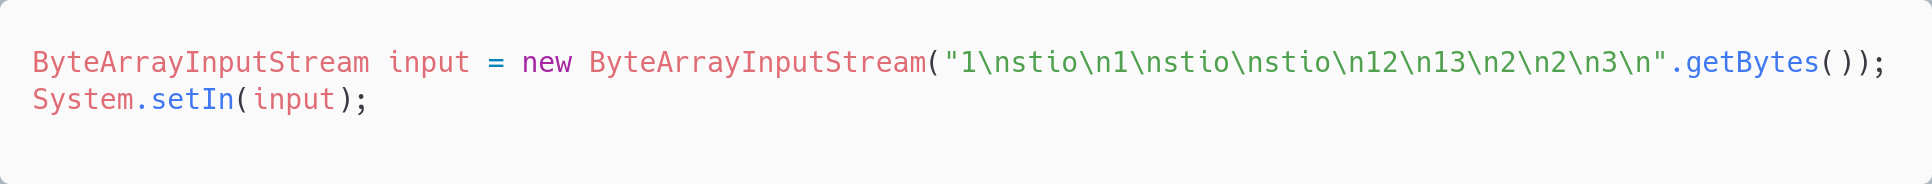
\includegraphics[width=1\linewidth]{testString.png}
    \caption{esempio di sequenza di input testata}
    \label{fig:testString}
  \end{figure}

  \subsubsection{HomeHandlerTest}

  \begin{itemize}

    \item \textbf{\textit{testHomeSearch()}}: verifica la navigazione dalla homepage alla pagina di ricerca, confrontando l'identificativo dell'ultimo Handler che ha chiamato l'\textit{update()} con quello di \textit{SearchHandler}

    \item \textbf{\textit{testHomeViewPlaylists()}}: verifica la navigazione dalla homepage alla pagina di visualizzazione delle playlist di un utente, confrontando l'identificativo dell'ultimo Handler che ha chiamato l'\textit{update()} con quello di \textit{UserPlaylistsHandler}

    \item \textbf{\textit{testHomeSuggestions()}}: verifica la navigazione dalla homepage alla pagina di visualizzazione dei suggeriti, confrontando l'identificativo dell'ultimo Handler che ha chiamato l'\textit{update()} con quello di \textit{SuggestionHandler}

  \end{itemize}

  \subsubsection{PlaybackHandlerTest}
  \begin{itemize}

    \item \textbf{\textit{testInitialPlaybackState()}}: verifica che lo stato iniziale della coda di riproduzione sia corretto. In particolare,
    dopo aver inserito una canzone \textit{song} nella coda di riproduzione, verifica che il thread in esecuzione rappresentante la coda stessa sia attivo (con il metodo \textit{Thread.isAlive()}) e che \textit{song} sia in pausa

    \item \textbf{\textit{testPlayPauseFunctionality()}}: verifica la funzionalità di pausa di una canzone, controllando se il thread relativo alla coda sia in esecuzione (se una canzone è in riproduzione) oppure no

    \item \textbf{\textit{testSkipFunctionality()}}: verifica la funzionalità di skip di una canzone

    \item \textbf{\textit{testTrackSwitching()}}: verifica che la coda di riproduzione passi correttamente da una canzone in riproduzione alla successiva; in particolare, controlla che la successiva canzone nella coda sia in riproduzione dopo che quella corrente è terminata

  \end{itemize}

  \subsubsection{RegistrationLoginHandlersTest}
  \begin{itemize}
    \item \textbf{\textit{testRegistrationCustomer()}}:
    dopo aver aggiunto un utente (oggetto di tipo \textit{Customer}) al database, verifica che sia effettivamente presente attraverso \textit{CustomerDAO.getByUsername()} e che ce ne sia uno solo

    \item \textbf{\textit{testRegistrationArtist()}}:
    dopo aver aggiunto un artista (oggetto di tipo \textit{Artist}) al database, verifica che sia effettivamente presente attraverso \textit{ArtistDAO.getByUsername()} e che ce ne sia uno solo

    \item \textbf{\textit{testLoginCustomer()}}: dopo aver aggiunto un utente (oggetto di tipo \textit{Customer}) al database e dopo aver fatto registrazione e login, verifica che nome e password di tale utente corrispondano a quelli memorizzati nella sessione corrente

    \item \textbf{\textit{testLoginArtist()}}: dopo aver aggiunto un artista (oggetto di tipo \textit{Artist}) al database e dopo aver fatto registrazione e login, verifica che nome e password di tale artista corrispondano a quelli memorizzati nella sessione corrente

  \end{itemize}

  \subsubsection{AlbumLoadHandlerTest}
  \begin{itemize}
    \item \textbf{\textit{testSuccessfulAlbumLoad()}}: dopo aver creato un album contenente una sola canzone, verifica che tale canzone sia presente e che sia effettivamente l'unica al suo interno
  \end{itemize}



\end{document}
